\documentclass{beamer}
\usepackage{polyglossia}
\setdefaultlanguage{german}

\usepackage{amsmath}
\usepackage{amsthm}
\usepackage{unicode-math}
% try later
%\setmathfont{texgyrepagella-math.otf}
\usepackage{tikz}
\usetikzlibrary{automata, positioning}

\usetheme{Warsaw}

\newcommand\relphantom[1]{\mathrel{\phantom{#1}}}
\setcounter{secnumdepth}{-2}

\newtheorem{defi}{Definition}
\newtheorem{thm}{Theorem}
\newtheorem{lmm}{Lemma}
\newtheorem{fct}{Fakt}

\title{Zeitdiskrete Markowketten}
\author{Marcel Wienöbst}
\date{19.12.2017}
\begin{document}
\maketitle
\begin{frame}{Gambler's Ruin}
  \begin{itemize}
  \item Das Gambler's Ruin Problem wird auf dem Wertebereich $\{0,1,2,\dots\}$ betrachtet.
    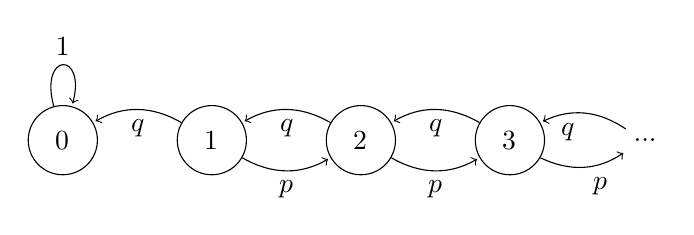
\begin{tikzpicture}
      % Add the states
      \node[state]             (zero) {$0$};
      \node[state, right=of zero] (one) {$1$};
      \node[state, right=of one] (two) {$2$};
      \node[state, right=of two] (three) {$3$};
      \node[right=of three] (dots) {...};
        
      % Connect the states with arrows
      \draw[every loop]
      (zero) edge[loop above]  node {1} (zero)
      (one) edge[bend right, auto=left] node {$q$} (zero)
      (one) edge[bend right, auto=right] node {$p$} (two)
      (two) edge[bend right, auto=left] node {$q$} (one)
      (two) edge[bend right, auto=right] node {$p$} (three)
      (three) edge[bend right, auto=left] node {$q$} (two)
      (three) edge[bend right, auto=right] node {$p$} (dots)
      (dots) edge[bend right, auto=left] node {$q$} (three);
    \end{tikzpicture}
  \item Zur Erinnerung: $A_k(1)$ ist die Wahrscheinlichkeit des Ruins (Absorption bei $x=0$, wenn mit Kapital $k$ gestartet wird).
  \item Weiterhin gilt: $A_k(t) = c_1 λ_1^k + c_2 λ_2^k$, aber nun $A_0(t) = 1$ und $\lim_{k→∞}|A_k(t)| < ∞$
  \end{itemize}
\end{frame}
\begin{frame}{Gambler's Ruin}
  \begin{itemize}
  \item Es folgt:
    \[
      a_k = A_k(1) =
      \begin{cases}
        1 &\text{wenn } p \leq q, \\
        (q/p)^k &\text{wenn } p > q
      \end{cases}
    \]
  \item Für die Dauer $τ_k$ bis zur Absorption ergibt sich
    \[
      τ_k =
      \begin{cases}
        k/(q-p), &\text{wenn } p < q, \\
        ∞, &\text{wenn } p \geq q.
      \end{cases}
    \]
  \end{itemize}
\end{frame}
\begin{frame}{Wiederholung}
  Eigenschaften von Markowketten:
  \begin{itemize}
  \item irreduzibel
  \item aperiodisch
  \item transient/rekurrent
  \item ergodisch
  \end{itemize}
\end{frame}
\begin{frame}{Stationäre Wahrscheinlichkeitsverteilungen}
  \begin{defi}
    Eine stationäre Wahrscheinlichkeitsverteilung einer Markowkette mit den Zuständen $\{1,2,...\}$   ist der nichtnegative Vektor $π = (π_1,π_2,...)^T$, der die Bedingungen $Pπ = π$ und $Σ_{i=1}^∞π_i = 1$ erfüllt.
  \end{defi}
  \begin{fct}
    Für endliche Markowketten existiert immer eine stationäre Verteilung.
  \end{fct}
\end{frame}
\begin{frame}
  \begin{thm}
    Eine Markowkette sei stark ergodisch mit den Zuständen
    $\{1,2,\dots\}$ und der Übergangsmatrix $P$. Dann existiert eine
    eindeutige stationäre Verteilung $π = (π_1,π_2,\dots)^T$, $Pπ = π$,
    sodass
    \[
      \lim_{n →∞}p_{ij}^{(n)} = π_i, \text{ für } i,j=1,2,\dots
    \]
  \end{thm}
  \begin{itemize}
    \item Beweis kann bei Karlin und Taylor (1975) nachgelesen werden.
  \end{itemize}
\end{frame}
\begin{frame}{Weitere Eigenschaften endlicher Markowketten}
  \begin{thm}
    In einer endlichen Markowkette kann es keine
    null rekurrenten Zustände geben und nicht alle Zustände
    können transient sein. Daher ist jede endliche, irreduzible Markowkette positiv
    rekurrent.  
  \end{thm}
  Dazu:
  \begin{lmm}
    Ist $j$ ein transienter Zustand einer Markowkette und $i$ ein
    beliebiger Zustand der Markowkette, dann gilt:
    \[
      \lim_{n→∞} p_{ji}^{(n)} = 0
    \]
  \end{lmm}
\end{frame}
\begin{frame}{Weitere Eigenschaften endlicher Markowketten}
  \begin{itemize}
  \item Wir definieren die Matrix der erwarteten Ersteintrittszeiten bzw{.} Wiederkehrzeiten als:
    \[
      M = (μ_{ij}) = \begin{pmatrix}
        μ_{11} & μ_{12} & \dots & μ_{1N} \\
        μ_{21} & μ_{22} & \dots & μ_{2N} \\
        \vdots & \vdots & \dots & \vdots \\
        μ_{N1} & μ_{N2} & \dots & μ_{NN}
      \end{pmatrix}
    \]
  \item Bei einer naiven Berechnungsmethode von $M$ müssten die Wahrscheinlichkeiten $\{f_{ii}^{(n)}\}$ und $\{f_{ji}^{(n)}\}$ betrachtet werden.
  \item Stattdessen können die folgenden Gleichungen aufgestellt werden:
    \[
      μ_{ji} = p_{ji} + Σ_{k=1,k≠j}^Np_{ki}(1+μ_{jk}) = 1+Σ_{k=1,k≠j}^Np_{ki}μ_{jk}.
    \]
  \item In Matrixform:
    \[
      M = 1_{\{N,N\}} + (M - \text{diag}(M))P
    \]
  \end{itemize}
\end{frame}
\begin{frame}{Geburts- und Todesprozesse}
  \begin{itemize}
  \item Modellierung einer Population durch eine diskrete Markowkette, wobei der Zustand $X_n$ die Größe der Population nach $n$ Schritten angibt.
  \item Zwei Fälle:
    \begin{enumerate}
    \item Die Population ist begrenzt: $X_n \in \{0,1,2,\dots,N\}$.
    \item Die Population ist unbegrenzt: $X_n \in \{0,1,2,\dots\}$.
    \end{enumerate}
  \item In jedem Schritt $n → n+1$ eine Geburt, einen Tod oder eine unveränderte Populationsgröße.
  \item $b_i$ ist die Wahrscheinlichkeit einer Geburt, $d_i$ die Wahrscheinlichkeit eines Todes. Dabei gibt $i$ die Populationsgröße an. Wir setzen $b_0 = d_0 = 0$ und bei einer beschränkten Population $b_N = 0$.
  \end{itemize}
\end{frame}
\begin{frame}{Geburts- und Todesprozesse}
  \begin{itemize}
  \item Es sind also die Übergangswahrscheinlichkeiten folgendermaßen definiert:
    \begin{align*}
  p_{ji} &= \text{Prob}\{X_{n+1} = j | X_n = i\} \\
         &= \begin{cases}
           b_i &\text{für } j = i+1 \\
           d_i &\text{für } j = i-1 \\
           1 - (b_i+d_i) &\text{für } j = i \\
           0 &\text{für } j \neq i-1,i,i+1
         \end{cases}
    \end{align*}
  \item  Die Übergangsmatrix sieht damit folgendermaßen aus:
    \[
      P = \begin{pmatrix}
        1 & d_1 & \dots & 0 & 0 \\
        0 & 1 - (b_1 + d_1) &  \dots & 0 & 0 \\
        0 & b_1 & \dots & 0 & 0 \\
        \vdots & \vdots & \vdots & \vdots & \vdots \\
        0 & 0  &  \dots & 1 - (b_{N-1} + d_{N-1}) & d_N \\
        0 & 0  &  \dots & b_{N-1} & 1 - d_N \\
      \end{pmatrix}
    \]
  \end{itemize}
\end{frame}
\begin{frame}{Geburts- und Todesprozesse}
  \begin{itemize}
  \item Als gerichteter Graph ergibt sich:
    \begin{tikzpicture}
      % Add the states
      \node[state]             (zero) {$0$};
      \node[state, right=of zero] (one) {$1$};
      \node[state,right=of two] (dots) {$\dots$};
      \node[state,right=of dots] (ult) {$N$};
        
      % Connect the states with arrows
      \draw[every loop]
      (zero) edge[loop above]  node {1} (zero)
      (one) edge[bend right, auto=left] node {$d_1$} (zero)
      (one) edge[bend right, auto=right] node {$b_1$} (dots)
      (one) edge[loop above] node {$1-(b_{1}+d_{1})$} (one)
      (dots) edge[bend right, auto=left] node {$d_{2}$} (one)
      (dots) edge[bend right, auto=right] node {$b_{N-1}$} (ult)
      (ult) edge[bend right, auto=left] node {$d_N$} (dots)
      (ult) edge[loop above] node {$1-d_{N}$} (ult);
    \end{tikzpicture}
  \item Es gibt zwei kommunizierende Klassen $\{0\}$ und $\{1,2,\dots,N\}$. Dabei ist $\{0\}$ positiv rekurrent und alle weiteren Zustände sind transient.
  \item Es existiert eine
    eindeutige stationäre Verteilung $π$, wobei $π_0 = 1$ und $π_i = 0$
    für $i = 1,2,\dots,N$. Außerdem gilt
    \[
      \lim_{n→∞} P(X_n = 0) = \lim_{n→∞}p_0(n) = 1.
    \]
  \end{itemize}
\end{frame}
\begin{frame}{Geburts- und Todesprozesse}
  \begin{itemize}
  \item Wie lange dauert es bis die Population ausstirbt?
  \item Dazu sei $τ_k$ die erwartete Aussterbedauer für eine Population der Größe $k$. Damit ist $τ_0 = 0$, für $0 < k < N$
    \[
      τ_k = b_k(1+τ_{k+1}) + d_k(1 + τ_{k-1}) + (1-(b_k + d_k))(1+τ_k).
    \]
    und $τ_N = d_N(1+τ_{N-1}) + (1-d_N)(1+τ_N)$.
  \item Diese Differenzengleichung kann vereinfacht werden zu:
    \[
      d_kτ_{k-1} - (b_k+d_k)τ_k + b_kτ_{k+1} = -1
    \]
    für $k = 1,2,\dots,N-1$. Für $k = N$ ergibt sich $d_Nτ_{N-1} - d_Nτ_N = -1$.
  \end{itemize}
\end{frame}
\begin{frame}{Geburts- und Todesprozesse}
  \begin{itemize}
    \item Diese Differenzengleichungen können als Matrixgleichung $Dτ = c$ interpretiert werden, wobei $τ =
    (τ_0,τ_1,\dots,τ_N)^T$, $c = (0,-1,\dots,-1)^T$ und
    \begin{align*}
      D &=
  \begin{pmatrix}
    1 & 0 & 0 & 0 & \cdots & 0 & 0 \\
    d_1 & -b_1-d_1 & b_1 & 0 & \cdots & 0 & 0 \\
    0 & d_2 & -b_2-d_2 & b_2 & \cdots & 0 & 0 \\
    \vdots & \vdots & \vdots & \vdots & \vdots & \vdots & \vdots \\
    0 & 0 & 0 & 0 & \cdots & d_N & -d_N 
  \end{pmatrix} \\
        &= \begin{pmatrix}
      1 & 0 \\
      D_1 & D_N
    \end{pmatrix}
    \end{align*}
  \item Es kann gezeigt werden, dass $\det(D_N) ≠ 0$. Da $\det(D) = \det(D_N)$ gilt, ist $D$ invertierbar und es folgt: $τ = D^{-1}c$.
  \end{itemize}
\end{frame}
\begin{frame}{Geburts- und Todesprozesse}
  \begin{itemize}
  \item Es kann auch eine analytische Lösung für die erwartete Zeit bis zum Aussterben der Population gefunden werden (Nisbet und Gurney [1982]).
  \end{itemize}
  \begin{thm}
    Für einen wie zuvor beschriebenen Geburts- und Todesprozess $\{X_n\}$ ergibt sich als erwartet Zeit bis zum Aussterben bei einer Startpopulation der Größe $m$:
    \[
      τ_m = \begin{cases}
        1/d_1 + Σ_{i=2}^N \frac{b_1\cdots b_{i-1}}{d_1, \cdots, d_i}, &m = 1 \\
        τ_1 + Σ_{s=1}^{m-1}\left(\frac{d_1\cdots d_s}{b_1\cdots b_s} Σ_{i = s+1}^N \frac{b_1\cdots b_{i-1}}{d_1\cdots d_i}\right), &m = 2, \dots N.
      \end{cases}
    \]
  \end{thm}
\end{frame}
\begin{frame}{Logistische Wachstumsprozesse}
  \begin{itemize}
  \item Wir wählen nun $b_i$ und $d_i$, sodass der Geburts- und Todesprozess logistische Form hat.
  \item Deterministisches logistisches Modell:
    \[
      \frac{dy}{dt} = ry(1-\frac{y}{K}), \; y(0) = y_0 > 0,
    \]
    wobei $y(t)$ die Populationsgröße nach Zeit $t$ beschreibt. Dabei ist $r$ der Wachstumsfaktor und $K$ eine obere Schranke für $y(t)$.
  \item Wir machen für den logistischen Wachstumsprozess die Annahme:
    \[
      b_i - d_i = ri(1-i/K),
    \]
    für $i=0,1,2,\dots,N$, wobei $N > K$.
  \item Die erwartete Zeit bis zum Aussterben der Population kann, wie zuvor hergeleitet, berechnet werden.
  \end{itemize}
\end{frame}
\begin{frame}{Logistische Wachstumsprozesse}
  \begin{itemize}
  \item Wir betrachten zwei Möglichkeiten $b_i$ und $d_i$ entsprechend der obigen Bedingung zu wählen:
    \begin{enumerate}
    \item \[b_i = r(i - \frac{i^2}{2K}) \text{ und } d_i = r\frac{i^2}{2K}, \; i = 0,1,2,\dots,2K \]
    \item \[b_i = \begin{cases} ri,  &i = 0,1,2,\dots,N-1 \\ 0, &i \geq N \end{cases} \text{ und } d_i = r\frac{i^2}{K}, i = 0,1,\dots,N\]
    \end{enumerate}
  \end{itemize}
\end{frame}
\begin{frame}{Quasistationäre Verteilung}
  \begin{itemize}
  \item Wie verhält sich ein Geburts- und Todesprozess (und speziell der logistische Wachstumsprozess) unter der Annahme des Nicht-Aussterbens?
  \item Sei $\{X_n\}$ für $n = 0,1,2,\dots,N$ ein Geburts- und Todesprozess mit $p_i(n) = P(X_n=i\}, i = 0,1,2,\dots,N$. Wir definieren für $i = 1,2,\dots,N$ die bedingte Wahrscheinlichkeit:
    \begin{align*}
      q_i(n) &= P(X_n=i|X_j \neq 0, j = 0,1,2,\dots,n-1) \\
             &= \frac{p_i(n)}{1-p_0(n)}
    \end{align*}
  \item Dabei ist $q(n) = (q_1(n),q_2(n), \dots, q_N(n))^T$ eine Wahrscheinlichkeitsverteilung.
  \end{itemize}
\end{frame}
\begin{frame}{Quasistationäre Verteilung}
  \begin{itemize}
  \item Wir betrachten nun die Markowkette $\{Q_n\}$, wobei $Q_n$ die Zufallsvariable der Populationsgröße zum Zeitpunkt $n$ sei: $P(Q_n = i) = q_i(n)$.
  \item Die stationäre Verteilung $q*$ dieses Prozesses wird quasistationäre Verteilung genannt.
  \item Wir stellen die Differenzengleichung für $q_i(n+1)$ auf:
    \begin{align*}
      q_i(n+1) &= \frac{p_i(n+1)}{1-p_0(n+1)} \\
               &= \left(\frac{p_i(n+1)}{1-p_0(n)}\right)\left(\frac{1-p_0(n)}{1-p_0(n+1)}\right) \\
               &= \left(\frac{p_i(n+1)}{1-p_0(n)}\right)\left(\frac{1-p_0(n)}{1-p_0(n)-d_1p_1(n)}\right)
    \end{align*}
  \end{itemize}
\end{frame}
\begin{frame}{Quasistationäre Verteilung}
  \begin{itemize}
  \item Und damit:
    \begin{align*}
      q_i(n+1)(1-d_1q_1(n)) &= \left(\frac{p_i(n+1)}{1-p_0(n)}\right) \\
                            &= b_{i-1}q_{i-1}(n) + (1-b_i-d_i)q_i(n) \\
                            &\relphantom{=}{} + d_{i+1}q_{i+1}(n)
    \end{align*}
   \item Als Approximation nehmen wir an, dass $d_1 = 0$:
     \[
       \bar{q}_i(n+1) = b_{i-1}\bar{q}_{i-1}(n) + (1 - b_i - d_i)\bar{q}_i(n) + d_{i+1}\bar{~}{q}_{i+1}(n)
     \]
     für $i = 2,\dots, N-1$. Für $i = 1$ bzw{.} $i = N$:
     \[
       \bar{q}_1(n+1) = (1 - b_1)\bar{q}_1(n) + d_2\bar{q}_2(n)
     \]
     und
     \[
       \bar{q}_N(n+1) = b_{N-1}\bar{q}_{N-1}(n) + (1-d_N)\bar{q}_N(n).
     \]
  \end{itemize}
\end{frame}
\begin{frame}{Quasistationäre Verteilung}
  \begin{itemize}
  \item Die zu dieser Approximation gehörige Übergangsmatrix $\bar{P}$ ist eine Submatrix von $P$, wobei $d_1 = 0$.
      \[
      \bar{P} = \begin{pmatrix}
        1-b_1 & d_2 & \dots & 0 & 0 \\
        b_1 & 1 - (b_2 + d_2) &  \dots & 0 & 0 \\
        0 & b_2 & \dots & 0 & 0 \\
        \vdots & \vdots & \vdots & \vdots & \vdots \\
        0 & 0  &  \dots & 1 - (b_{N-1} + d_{N-1}) & d_N \\
        0 & 0  &  \dots & b_{N-1} & 1 - d_N \\
      \end{pmatrix}
    \]
  \item Die Markowkette ist ergodisch (irreduzibel, positiv rekurrent und aperiodisch) und hat eine eindeutige stationäre Wahrscheinlichkeitsverteilung $\bar{q}^*$, $\bar{P}\bar{q}^* = \bar{q}^*$.
  \item Es gilt:
    \[
      \bar{q}^*_{i+1} = \frac{b_i \cdots b_1}{d_{i+1}\cdots d_2}\bar{q}^*_{i}
    \]
  \end{itemize}
\end{frame}
\end{document}